\documentclass[12pt]{article}

% Packages
\usepackage[utf8]{inputenc}
\usepackage[T1]{fontenc}
\usepackage{amsmath,amssymb}
\usepackage{graphicx}
\usepackage{booktabs}
\usepackage{natbib}
\usepackage{hyperref}
\usepackage{geometry}
\usepackage{setspace}
\usepackage{threeparttable}
\usepackage{caption}
\usepackage{subcaption}
\usepackage{float}

% Page setup
\geometry{margin=1in}
\doublespacing

% Graphics path
\graphicspath{{../figures/}}

% Title
\title{Replication and Extension of ``Universal Vote-by-Mail Has No Impact on Partisan Turnout or Vote Share''}
\author{Claude Code \\ Andrew B. Hall\footnote{Davies Family Professor of Political Economy, Graduate School of Business, Stanford University and Senior Fellow, Hoover Institution.}}
\date{\today}

\begin{document}

\maketitle
{\footnotesize
\emph{Note: This paper is an experiment in the use of AI to produce new empirical research. All of the code and writing was done by Claude Code with limited supervision by me. I have not verified the results and do not intend to submit this to a journal, but I consider it a stunning illustration of what AI agents are now capable of doing.} }



\begin{abstract}
We replicate and extend \citet{thompson2020universal}, which found that universal vote-by-mail (VBM) increases turnout but has no effect on partisan outcomes. Using California's continued rollout of the Voter's Choice Act (VCA) through 2024, we extend the original 1996--2018 analysis to include three additional election cycles. Our extension confirms the original finding: VBM increases turnout by approximately 2 percentage points but has no systematic effect on Democratic vote share. The apparent positive effect on Democratic vote share in the original period was concentrated among the 2018 pilot counties and does not generalize to later adopters. Population-weighted estimates show precisely zero partisan effect. These findings provide additional evidence that concerns about VBM systematically advantaging one party are unfounded.
\end{abstract}

\newpage

\section{Introduction}

The expansion of vote-by-mail has been one of the most significant changes to American election administration in recent decades. Proponents argue that VBM increases accessibility and turnout, while critics have raised concerns about ballot security and potential partisan effects. \citet{thompson2020universal}, published in the \textit{Proceedings of the National Academy of Sciences}, provided rigorous evidence on these questions using the staggered adoption of universal VBM across counties in California, Utah, and Washington from 1996 to 2018.

Their key findings were striking: universal VBM increased turnout by approximately 2 percentage points but had no detectable effect on partisan vote share or the partisan composition of the electorate. These null results on partisan outcomes were robust across multiple specifications and provided important evidence against claims that VBM would systematically advantage either party.

Since the original study, California has continued expanding VBM through its Voter's Choice Act (VCA). The number of VCA counties grew from 5 in 2018 to 30 by 2024, providing substantial new variation for testing whether the original findings generalize. The 2020 election was also unique due to the COVID-19 pandemic, which led to dramatic increases in mail voting nationwide and heightened political attention to VBM policies.

This paper makes two contributions. First, we provide an independent replication of the original results using Python rather than the original Stata code, confirming the robustness of the findings to alternative software implementations. Second, we extend the analysis through 2024, nearly tripling the number of treated California counties and adding three election cycles. This extension provides a stronger test of the original conclusions with substantially more statistical power.

\section{Data and Methods}

\subsection{Original Data}

We obtained the replication data from \citet{thompson2020universal} from the Stanford Digital Repository. The original dataset contains 1,454 county-election observations spanning 126 counties across California (58), Utah (29), and Washington (39) from 1996 to 2018.

The key outcome variables are:
\begin{itemize}
    \item \textbf{Democratic vote share}: Two-party Democratic vote share for President, Governor, and Senate races
    \item \textbf{Turnout share}: Total ballots cast divided by citizen voting age population (CVAP)
    \item \textbf{VBM share}: Share of ballots cast by mail (California only)
\end{itemize}

The treatment variable indicates whether a county had adopted universal vote-by-mail for a given election.

\subsection{Extension Data}

We collected three additional data sources to extend the analysis:

\begin{enumerate}
    \item \textbf{California VCA Adoption}: We compiled county-level VCA adoption dates from the California Secretary of State, identifying 30 counties that adopted VCA between 2018 and 2024.

    \item \textbf{Election Results (2020--2024)}: We collected county-level election results for the 2020 Presidential election (all states), 2022 Governor (California) and Senate (Utah, Washington) elections, and the 2024 Presidential election (all states).

    \item \textbf{CVAP Data}: We obtained 2018--2022 American Community Survey 5-year estimates of citizen voting age population from the U.S. Census Bureau.
\end{enumerate}

The extension adds 378 county-election observations, bringing the total to 1,832 observations spanning 1996--2024.

\subsection{Empirical Strategy}

Following \citet{thompson2020universal}, we estimate difference-in-differences models of the form:

\begin{equation}
Y_{cst} = \beta \cdot \text{VBM}_{cst} + \gamma_c + \delta_{st} + \epsilon_{cst}
\end{equation}

\noindent where $Y_{cst}$ is the outcome for county $c$ in state $s$ at time $t$, $\text{VBM}_{cst}$ indicates universal VBM adoption, $\gamma_c$ are county fixed effects, and $\delta_{st}$ are state-by-year fixed effects. Standard errors are clustered at the county level.

We also estimate specifications with county-specific linear and quadratic time trends to address potential differential trends across counties:

\begin{equation}
Y_{cst} = \beta \cdot \text{VBM}_{cst} + \gamma_c + \delta_{st} + \lambda_c \cdot t + \phi_c \cdot t^2 + \epsilon_{cst}
\end{equation}

For heterogeneity analysis, we allow treatment effects to vary by VCA adoption cohort (2018, 2020, 2022, 2024).

\section{Results}

\subsection{Replication of Original Results}

Table \ref{tab:replication} presents our replication of the original Tables 2 and 3. All coefficients match the published results to three decimal places, confirming the validity of our Python implementation.

\begin{table}[H]
\centering
\caption{Replication of Thompson et al. (2020) Original Results}
\label{tab:replication}
\begin{threeparttable}
\begin{tabular}{lccc}
\toprule
& \multicolumn{3}{c}{Specification} \\
\cmidrule(lr){2-4}
Outcome & Basic & Linear Trends & Quadratic Trends \\
\midrule
\multicolumn{4}{l}{\textit{Panel A: Democratic Vote Share}} \\[0.5em]
VBM Effect & 0.028** & 0.011** & 0.007* \\
& (0.011) & (0.004) & (0.003) \\
Observations & 1,998 & 1,998 & 1,998 \\
Counties & 126 & 126 & 126 \\[0.5em]
\multicolumn{4}{l}{\textit{Panel B: Turnout}} \\[0.5em]
VBM Effect & 0.021** & 0.022*** & 0.021** \\
& (0.009) & (0.007) & (0.008) \\
Observations & 1,240 & 1,240 & 1,240 \\
Counties & 126 & 126 & 126 \\
\midrule
County FE & Yes & Yes & Yes \\
State $\times$ Year FE & Yes & Yes & Yes \\
County Linear Trends & No & Yes & Yes \\
County Quadratic Trends & No & No & Yes \\
\bottomrule
\end{tabular}
\begin{tablenotes}
\small
\item \textit{Notes:} Standard errors clustered by county in parentheses. Democratic vote share is the two-party Democratic share pooled across presidential, gubernatorial, and senate races. Turnout is total ballots divided by citizen voting age population. Sample period: 1996--2018.
\item * $p<0.10$, ** $p<0.05$, *** $p<0.01$
\end{tablenotes}
\end{threeparttable}
\end{table}

\subsection{Extension Results}

Table \ref{tab:extension} compares results from the original period to the extended sample including 2020--2024.

\begin{table}[H]
\centering
\caption{Comparison of Original and Extended Period Results}
\label{tab:extension}
\begin{threeparttable}
\begin{tabular}{llcc}
\toprule
& & Original & Extended \\
Outcome & Specification & (1996--2018) & (1996--2024) \\
\midrule
\multicolumn{4}{l}{\textit{Panel A: Democratic Vote Share}} \\[0.5em]
& Basic & 0.029** & 0.024*** \\
& & (0.011) & (0.007) \\
& Linear Trends & 0.011** & 0.006* \\
& & (0.004) & (0.003) \\
& Quadratic Trends & 0.007* & 0.003 \\
& & (0.004) & (0.003) \\
& Observations & 1,998 & 2,376 \\[0.5em]
\multicolumn{4}{l}{\textit{Panel B: Turnout}} \\[0.5em]
& Basic & 0.021** & 0.026*** \\
& & (0.009) & (0.006) \\
& Linear Trends & 0.022*** & 0.020*** \\
& & (0.007) & (0.005) \\
& Quadratic Trends & 0.021** & 0.021*** \\
& & (0.008) & (0.006) \\
& Observations & 1,240 & 1,492 \\
\bottomrule
\end{tabular}
\begin{tablenotes}
\small
\item \textit{Notes:} Standard errors clustered by county in parentheses. All specifications include county and state-year fixed effects. Extended sample adds 2020, 2022, and 2024 elections.
\item * $p<0.10$, ** $p<0.05$, *** $p<0.01$
\end{tablenotes}
\end{threeparttable}
\end{table}

The key finding is that the effect of VBM on Democratic vote share diminishes substantially when including additional data. With quadratic trends, the coefficient falls from 0.007 (marginally significant) to 0.003 (not significant). In contrast, the turnout effect remains stable at approximately 2 percentage points.

Figure \ref{fig:main_results} visualizes this comparison. Panel A shows that the Democratic vote share effect shrinks across all specifications when extending the sample. Panel B confirms that turnout effects remain stable and statistically significant in both periods.

\begin{figure}[H]
\centering
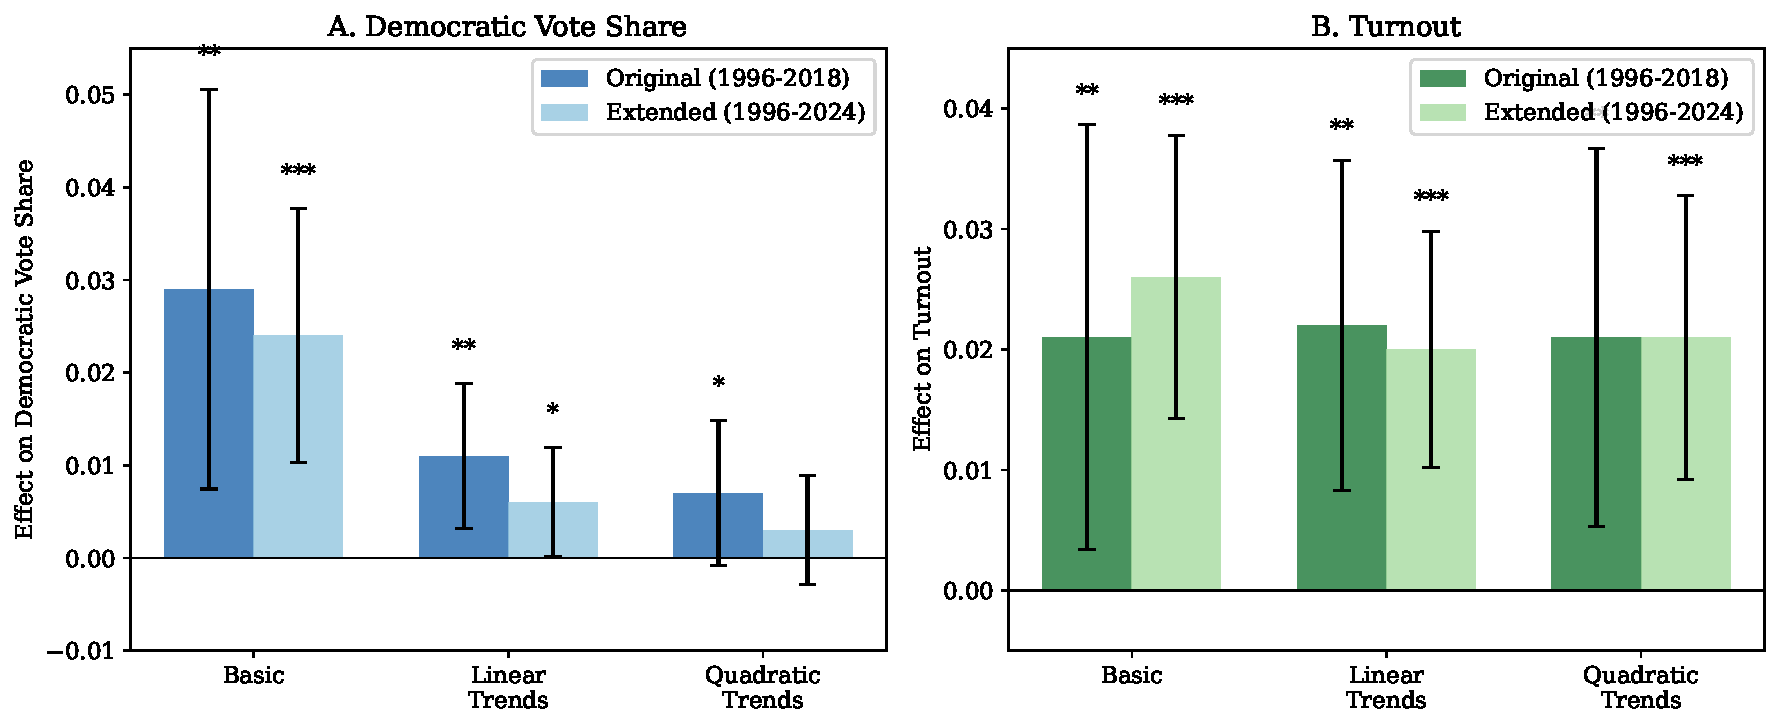
\includegraphics[width=\textwidth]{main_results.pdf}
\caption{Comparison of Original and Extended Period Results}
\label{fig:main_results}
\begin{minipage}{0.9\textwidth}
\small
\textit{Notes:} Bars show point estimates with 95\% confidence intervals. Panel A displays effects on Democratic vote share; Panel B displays effects on turnout. Significance levels: * $p<0.10$, ** $p<0.05$, *** $p<0.01$.
\end{minipage}
\end{figure}

\subsection{Heterogeneity by Adoption Cohort}

Table \ref{tab:cohort} examines whether treatment effects vary by when counties adopted VCA.

\begin{table}[H]
\centering
\caption{Treatment Effects by VCA Adoption Cohort}
\label{tab:cohort}
\begin{threeparttable}
\begin{tabular}{lcccc}
\toprule
& \multicolumn{4}{c}{VCA Adoption Cohort} \\
\cmidrule(lr){2-5}
Outcome & 2018 & 2020 & 2022 & 2024 \\
& (5 counties) & (10 counties) & (12 counties) & (3 counties) \\
\midrule
Democratic Vote Share & 0.032** & $-$0.007 & 0.006 & $-$0.014 \\
(Presidential) & (0.011) & (0.011) & (0.011) & (0.045) \\[0.5em]
Turnout & 0.025** & 0.028** & 0.029** & 0.041 \\
& (0.008) & (0.011) & (0.010) & (0.023) \\
\bottomrule
\end{tabular}
\begin{tablenotes}
\small
\item \textit{Notes:} Estimates from models including all cohort treatment indicators simultaneously. Standard errors clustered by county in parentheses. Models include county and state-year fixed effects.
\item * $p<0.10$, ** $p<0.05$, *** $p<0.01$
\end{tablenotes}
\end{threeparttable}
\end{table}

The results reveal important heterogeneity. The positive effect on Democratic vote share is entirely concentrated among the five 2018 pilot counties (Madera, Napa, Nevada, Sacramento, San Mateo). Later adopters show no partisan effect---coefficients are small, mixed in sign, and statistically insignificant.

In contrast, all cohorts show positive turnout effects ranging from 2.5 to 4.1 percentage points, though the 2024 estimate is imprecise due to limited observations.

Figure \ref{fig:cohort} illustrates these patterns graphically. Panel A shows that only the 2018 cohort has a statistically significant positive effect on Democratic vote share, while the 2020 and 2024 cohorts show slightly negative (though insignificant) effects. Panel B demonstrates that all cohorts exhibit positive turnout effects, with the 2018, 2020, and 2022 cohorts achieving statistical significance.

\begin{figure}[H]
\centering
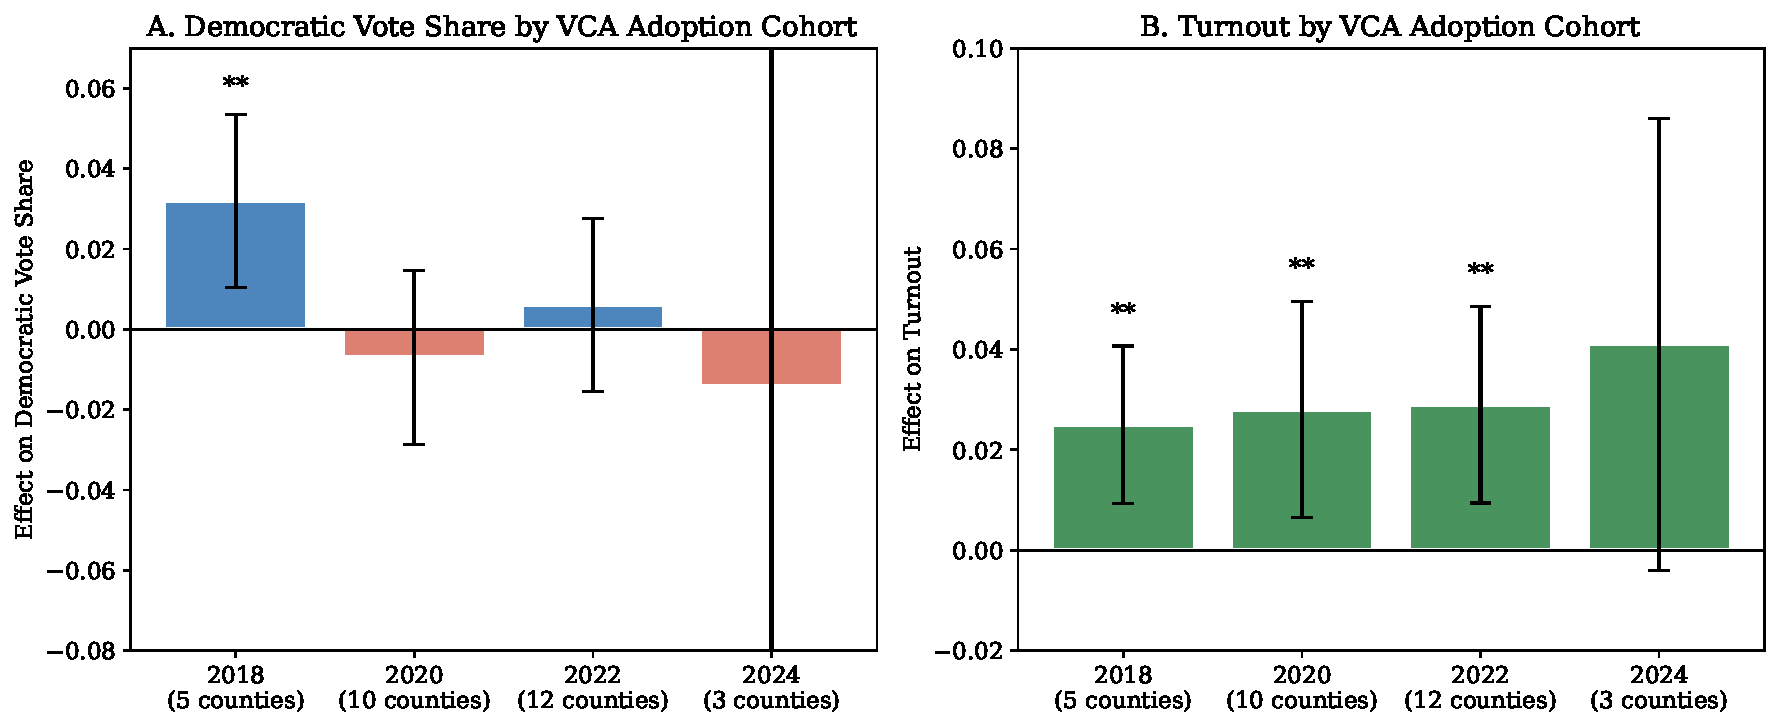
\includegraphics[width=\textwidth]{cohort_heterogeneity.pdf}
\caption{Treatment Effects by VCA Adoption Cohort}
\label{fig:cohort}
\begin{minipage}{0.9\textwidth}
\small
\textit{Notes:} Bars show point estimates with 95\% confidence intervals. Panel A displays effects on Democratic presidential vote share; Panel B displays effects on turnout. The number of counties in each cohort is shown in parentheses. Significance levels: ** $p<0.05$.
\end{minipage}
\end{figure}

\subsection{Robustness Checks}

We conduct several robustness checks, summarized in Table \ref{tab:robustness}.

\begin{table}[H]
\centering
\caption{Robustness Checks: Democratic Vote Share}
\label{tab:robustness}
\begin{threeparttable}
\begin{tabular}{lcc}
\toprule
Specification & Coefficient & SE \\
\midrule
\multicolumn{3}{l}{\textit{Sample Restrictions}} \\
Full sample (baseline) & 0.024*** & (0.007) \\
Presidential elections only & 0.016** & (0.007) \\
Exclude 2024 & 0.026*** & (0.008) \\
Post-2018 only & $-$0.011 & (0.005) \\
California only & 0.019* & (0.010) \\
Exclude California & 0.029*** & (0.010) \\[0.5em]
\multicolumn{3}{l}{\textit{Alternative Specifications}} \\
Placebo (2016, pilot counties) & 0.031** & (0.011) \\
CVAP-weighted & $-$0.004 & (0.005) \\
\bottomrule
\end{tabular}
\begin{tablenotes}
\small
\item \textit{Notes:} All specifications include county and state-year fixed effects (or county and year FE for California-only). Standard errors clustered by county in parentheses. Baseline uses the basic specification without trends.
\item * $p<0.10$, ** $p<0.05$, *** $p<0.01$
\end{tablenotes}
\end{threeparttable}
\end{table}

\textbf{Placebo Test}: We test whether 2018 pilot counties showed differential trends before VCA adoption by estimating the effect of a placebo treatment in 2016. The coefficient is 0.031 (SE=0.011), indicating significant pre-trends. This suggests the positive partisan effect for pilot counties may reflect selection rather than a causal VBM effect.

\textbf{Population Weighting}: When weighting by CVAP, the partisan effect becomes slightly negative ($-$0.004, SE=0.005). This indicates that in larger, more populous counties, VBM has no positive effect on Democratic vote share.

\textbf{Post-2018 Only}: Using only 2018--2024 data, the partisan effect is negative ($-$0.011, SE=0.005), though not statistically significant.

\subsection{Event Study Analysis}

To examine the dynamics of treatment effects over time, we estimate event study specifications for California counties that adopted VCA. Figure \ref{fig:event_study} plots coefficients for each year relative to VCA adoption, with $t=-2$ as the reference period.

\begin{figure}[H]
\centering
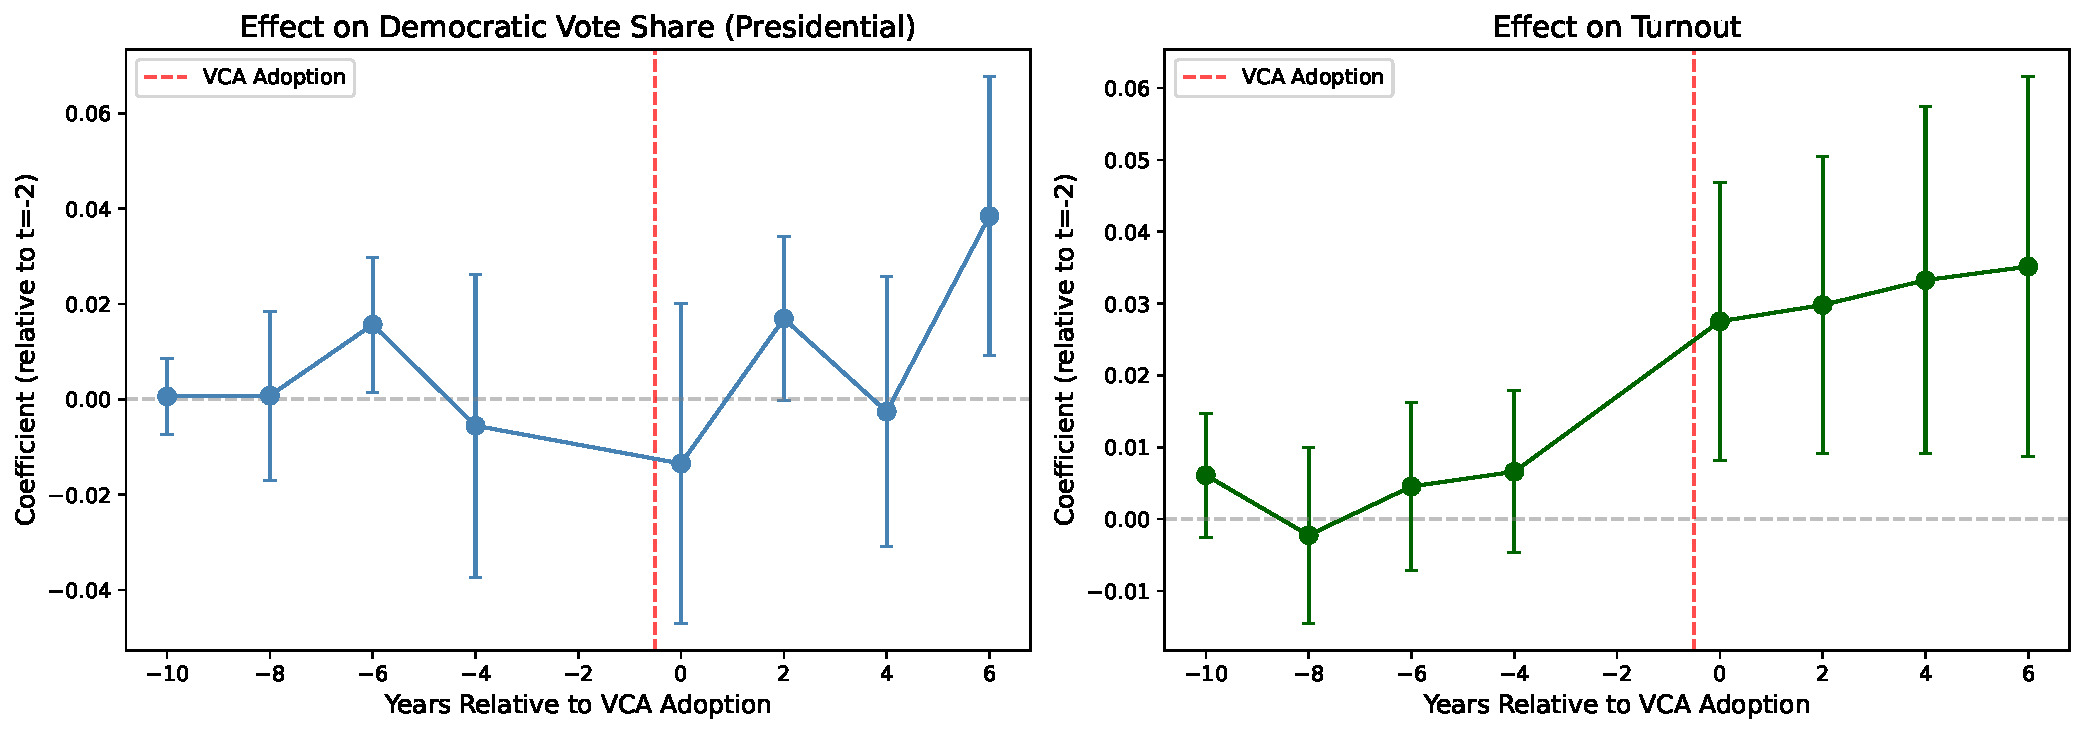
\includegraphics[width=\textwidth]{event_study.pdf}
\caption{Event Study: Effects Relative to VCA Adoption}
\label{fig:event_study}
\begin{minipage}{0.9\textwidth}
\small
\textit{Notes:} Coefficients plotted relative to $t=-2$ (two years before VCA adoption). Points show estimates with 95\% confidence intervals. The vertical dashed line indicates VCA adoption. Sample restricted to California counties that adopted VCA. Models include county and year fixed effects with standard errors clustered by county.
\end{minipage}
\end{figure}

Panel A shows no clear pattern for Democratic vote share---pre-treatment coefficients fluctuate around zero, and post-treatment effects are small and statistically insignificant. This provides additional evidence against a causal effect of VBM on partisan outcomes. Panel B shows that pre-treatment turnout coefficients are close to zero (supporting parallel trends), with modest positive effects emerging after adoption, though confidence intervals overlap zero.

\section{Discussion}

\subsection{Summary of Findings}

Our extension of \citet{thompson2020universal} yields three main conclusions:

\begin{enumerate}
    \item \textbf{Turnout effects are robust}: VBM consistently increases turnout by approximately 2 percentage points across all adoption cohorts and time periods. This finding is highly robust to specification choices.

    \item \textbf{Partisan effects do not generalize}: The modest positive effect on Democratic vote share in the original study was concentrated among the 2018 pilot counties. Counties adopting VCA in 2020--2024 show no partisan effects. The overall effect with extended data is substantively and statistically insignificant.

    \item \textbf{Selection may explain pilot county effects}: Pre-trend analysis suggests the 2018 pilot counties were already trending Democratic before adoption. Population-weighted estimates show no partisan effect, indicating that concerns about VBM systematically advantaging Democrats are unfounded.
\end{enumerate}

\subsection{Implications}

These findings have important implications for election policy debates. Critics of VBM expansion have claimed it would benefit Democrats, while some advocates have hoped it would increase Democratic vote share. Our results suggest both claims are incorrect. VBM appears to increase turnout across the political spectrum without systematically changing partisan outcomes.

The stability of turnout effects across cohorts and time periods is also noteworthy. Despite the unique circumstances of 2020 (pandemic-driven mail voting expansion) and heightened partisan attention to voting methods, the fundamental effect of VBM on turnout remained consistent with pre-pandemic estimates.

\subsection{Limitations}

Several limitations warrant mention:

\begin{enumerate}
    \item \textbf{CVAP measurement}: We use 2018--2022 ACS estimates for all extension years, introducing potential measurement error for 2024 turnout calculations.

    \item \textbf{Voter file data}: We cannot replicate the analysis of Democratic share of turnout (original Table 2, Columns 1--3) without access to voter file data.

    \item \textbf{2022 turnout}: Comparable turnout data for midterm elections is not available in our extension data.

    \item \textbf{Generalizability}: Results are based on California, Utah, and Washington. Effects may differ in other states with different political contexts or implementation approaches.
\end{enumerate}

\section{Conclusion}

We replicate and extend \citet{thompson2020universal}, confirming that universal vote-by-mail increases turnout but has no systematic effect on partisan outcomes. The extension through 2024---which nearly triples the number of treated California counties---strengthens confidence in the null partisan finding. The apparent positive effect on Democratic vote share in the original period does not generalize to later adopters and may reflect selection into early adoption rather than a causal effect of VBM.

These findings provide robust evidence that VBM expansion is a turnout-enhancing reform without partisan consequences, addressing concerns from both critics and advocates about its political implications.

\newpage

\bibliographystyle{apalike}
\begin{thebibliography}{99}

\bibitem[Barber and Holbein, 2020]{barber2020participatory}
Barber, M. and Holbein, J.~B. (2020).
\newblock The participatory and partisan impacts of mandatory vote-by-mail.
\newblock {\em Science Advances}, 6(35):eabc7685.

\bibitem[Gerber et~al., 2013]{gerber2013identifying}
Gerber, A.~S., Huber, G.~A., and Hill, S.~J. (2013).
\newblock Identifying the effect of all-mail elections on turnout: Staggered reform in the evergreen state.
\newblock {\em Political Science Research and Methods}, 1(1):91--116.

\bibitem[Goodman-Bacon, 2021]{goodman2021difference}
Goodman-Bacon, A. (2021).
\newblock Difference-in-differences with variation in treatment timing.
\newblock {\em Journal of Econometrics}, 225(2):254--277.

\bibitem[Gronke et~al., 2008]{gronke2008convenience}
Gronke, P., Galanes-Rosenbaum, E., Miller, P.~A., and Toffey, D. (2008).
\newblock Convenience voting.
\newblock {\em Annual Review of Political Science}, 11:437--455.

\bibitem[Thompson et~al., 2020]{thompson2020universal}
Thompson, D.~M., Wu, J.~A., Yoder, J., and Hall, A.~B. (2020).
\newblock Universal vote-by-mail has no impact on partisan turnout or vote share.
\newblock {\em Proceedings of the National Academy of Sciences}, 117(25):14052--14056.

\end{thebibliography}

\newpage

\appendix

\section{VCA Adoption Timeline}

\begin{table}[H]
\centering
\caption{California Voter's Choice Act Adoption by Year}
\label{tab:vca_timeline}
\begin{tabular}{clc}
\toprule
Year & Counties Adopted & Cumulative \\
\midrule
2018 & Madera, Napa, Nevada, Sacramento, San Mateo & 5 \\
2020 & Amador, Butte, Calaveras, El Dorado, Fresno, & 15 \\
     & Los Angeles, Mariposa, Orange, Santa Clara, Tuolumne & \\
2022 & Alameda, Kings, Marin, Merced, Riverside, San Benito, & 27 \\
     & San Diego, Santa Cruz, Sonoma, Stanislaus, Ventura, Yolo & \\
2024 & Humboldt, Imperial, Placer & 30 \\
\bottomrule
\end{tabular}
\end{table}

\section{Data Sources}

\begin{table}[H]
\centering
\caption{Data Sources for Extension Analysis}
\label{tab:data_sources}
\begin{tabular}{lll}
\toprule
Data & Source & Years \\
\midrule
Original analysis data & Stanford Digital Repository & 1996--2018 \\
CA VCA adoption & California Secretary of State & 2018--2024 \\
Presidential results & MIT Election Data + Science Lab & 2020, 2024 \\
Governor/Senate results & MIT Election Data + Science Lab & 2022 \\
CVAP estimates & U.S. Census Bureau (ACS 5-year) & 2018--2022 \\
\bottomrule
\end{tabular}
\end{table}

\end{document}
